% Common preamble for all lab reports
\documentclass[a4paper, 12pt]{article}

% Language and encoding
\usepackage[T2A]{fontenc}
\usepackage[utf8]{inputenc}
\usepackage[ukrainian]{babel}

% Typography
\usepackage{microtype}
\usepackage{lmodern}

% Page geometry
\usepackage[margin=25mm, headheight=14pt]{geometry}

% Math
\usepackage{amsmath, amssymb}

% Graphics and figures
\usepackage{graphicx}
\usepackage{float}
\usepackage{subcaption}
\usepackage[justification=centering]{caption}

% Tables
\usepackage{tabularx}
\usepackage{booktabs}
\usepackage{array}

% Colors and hyperlinks
\usepackage{xcolor}
\usepackage[colorlinks=true, linkcolor=blue!60!black, urlcolor=blue!60!black, citecolor=blue!60!black]{hyperref}

% Lists
\usepackage{enumitem}
\setlist{nosep, leftmargin=*}

% Section formatting
\usepackage{titlesec}
\titleformat{\section}{\large\bfseries}{\thesection.}{0.5em}{}
\titleformat{\subsection}{\normalsize\bfseries}{\thesubsection.}{0.5em}{}

% Header/footer
\usepackage{fancyhdr}
\pagestyle{fancy}
\fancyhf{}
\fancyhead[L]{\small\leftmark}
\fancyhead[R]{\small\thepage}
\renewcommand{\headrulewidth}{0.4pt}
\fancypagestyle{plain}{\fancyhf{}\fancyfoot[C]{\thepage}\renewcommand{\headrulewidth}{0pt}}

% Placeholder image command
\newcommand{\placeholder}[2][0.8\textwidth]{%
  \begin{figure}[H]
    \centering
    \fbox{\parbox{#1}{\vspace{4cm}\centering\textit{#2}\vspace{4cm}}}
    \caption{#2}
  \end{figure}
}

% Placeholder for inline result values
\newcommand{\result}[1]{\textbf{\textcolor{red!70!black}{[#1]}}}

\usepackage{../common/labstyle}

\labnum{1}
\labtitle{Мiцнiсний аналiз}

\begin{document}
\maketitle
\tableofcontents
\newpage

% ===================================================================
\section{Вихiднi данi}
% ===================================================================

Параметри моделi згiдно з варiантом~13:

\begin{table}[H]
  \centering
  \caption{Вихiднi данi (варiант~13)}
  \begin{tabularx}{0.75\textwidth}{Xr}
    \toprule
    \textbf{Параметр} & \textbf{Значення} \\
    \midrule
    Верхня кришка              & Плоска \\
    Нижня кришка               & Сферична \\
    Товщина стiнки             & 2{,}1~мм \\
    Внутрiшнiй тиск            & 1{,}1~МПа \\
    Робоча температура         & 75\textdegree C \\
    Зовнiшня висота ємностi    & 1000~мм \\
    Зовнiшнiй дiаметр ємностi  & 500~мм \\
    Матерiал                   & Stainless Steel \\
    \bottomrule
  \end{tabularx}
\end{table}

\subsection{Властивостi матерiалу Stainless Steel}

\begin{table}[H]
  \centering
  \begin{tabularx}{0.75\textwidth}{Xr}
    \toprule
    \textbf{Властивiсть} & \textbf{Значення} \\
    \midrule
    Density                    & 7750~кг/м$^3$ \\
    Young's Modulus            & 193~ГПа \\
    Poisson's Ratio            & 0{,}31 \\
    Tensile Yield Strength     & 207~МПа \\
    Tensile Ultimate Strength  & 586~МПа \\
    \bottomrule
  \end{tabularx}
\end{table}

\subsection{Ключовi формули}

Еквiвалентнi напруження за теорiєю Мiзеса:
\begin{equation}
  \sigma_{\mathrm{eq}} = \sqrt{\frac{1}{2}\left[
    (\sigma_1 - \sigma_2)^2 +
    (\sigma_2 - \sigma_3)^2 +
    (\sigma_3 - \sigma_1)^2
  \right]}.
\end{equation}

Повне перемiщення:
$U_{\mathrm{total}} = \sqrt{U_x^2 + U_y^2 + U_z^2}$.
Запас мiцностi:
$n = \sigma_{\mathrm{yield}} / \sigma_{\mathrm{eq}}$;
$n \geq 1$ --- конструкцiя витримує навантаження.

% ===================================================================
\section{Послiдовнiсть виконання}
% ===================================================================

Робота виконана у автоматизованому режимi через ANSYS Workbench Journaling (\texttt{lab1.wbjn}).

\begin{lstlisting}[style=scheme]
1. Geometry: CadQuery (geometry/lab1.py)
   |-- make_vessel_shell(): cyl. R=250mm, H=1000mm,
   |   wall=2.1mm, flat top + spherical bottom
   |-- make_support_pads(): 2 pads at 0/180 deg,
   |   50x250x10mm on outer wall at mid-height
   |-- Boolean Union -> single body
   |-- Export STEP -> geometry/step/lab1.step
2. ANSYS Workbench: CreateSystem("Static Structural")
3. Import lab1.step -> SpaceClaim
4. Enter Mechanical (Python via SendCommand)
   |-- Assign Stainless Steel to all bodies
   |-- ID bodies by volume: vessel=largest, pads=smaller
   |-- Mesh: element size 10mm
   |   -> 255048 nodes, 166461 elements
   |-- Fixed Support -> pad outer faces (r > 295mm)
   |-- Pressure 1.1 MPa -> vessel inner faces (r < 249mm)
   |-- Thermal Condition 75C (uniform, all bodies)
   |-- Gravity -Z = 9.807 m/s^2
   |-- Solve (PCG, 4 cores, 1729 iter, 64s)
   |-- Results: Total Deformation
   |-- Results: Equivalent Stress
   |-- Results: Equivalent Elastic Strain
   |-- Export images (PNG)
\end{lstlisting}

\subsection{Геометрiя (CadQuery $\to$ STEP)}

Параметричний скрипт \texttt{geometry/lab1.py} будує збiрку:
\begin{itemize}
  \item \textbf{vessel} --- цилiндрична оболонка ($R_{\mathrm{out}}=250$~мм, $h_{\mathrm{wall}}=2{,}1$~мм, $H=1000$~мм), плоска верхня кришка, сферична нижня кришка;
  \item \textbf{pads} --- 2 прямокутнi опори на цилiндричнiй стiнцi на половинi висоти ($50 \times 250 \times 10$~мм).
\end{itemize}
Експорт: \texttt{geometry/step/lab1.step}.

\subsection{Iдентифiкацiя тiл та граничнi умови}

Тiла iдентифiкуються за об'ємом: vessel (бiльший), pads (менший). Гранi vessel класифiкуються за радiусом центроїду: внутрiшнi ($r < 249$~мм) --- для тиску. Гранi pads: зовнiшнi ($r > 295$~мм) --- фiксована опора.

% ===================================================================
\section{Вiзуалiзацiя моделi}
% ===================================================================

\subsection{Геометрiя}

\begin{figure}[H]
  \centering
  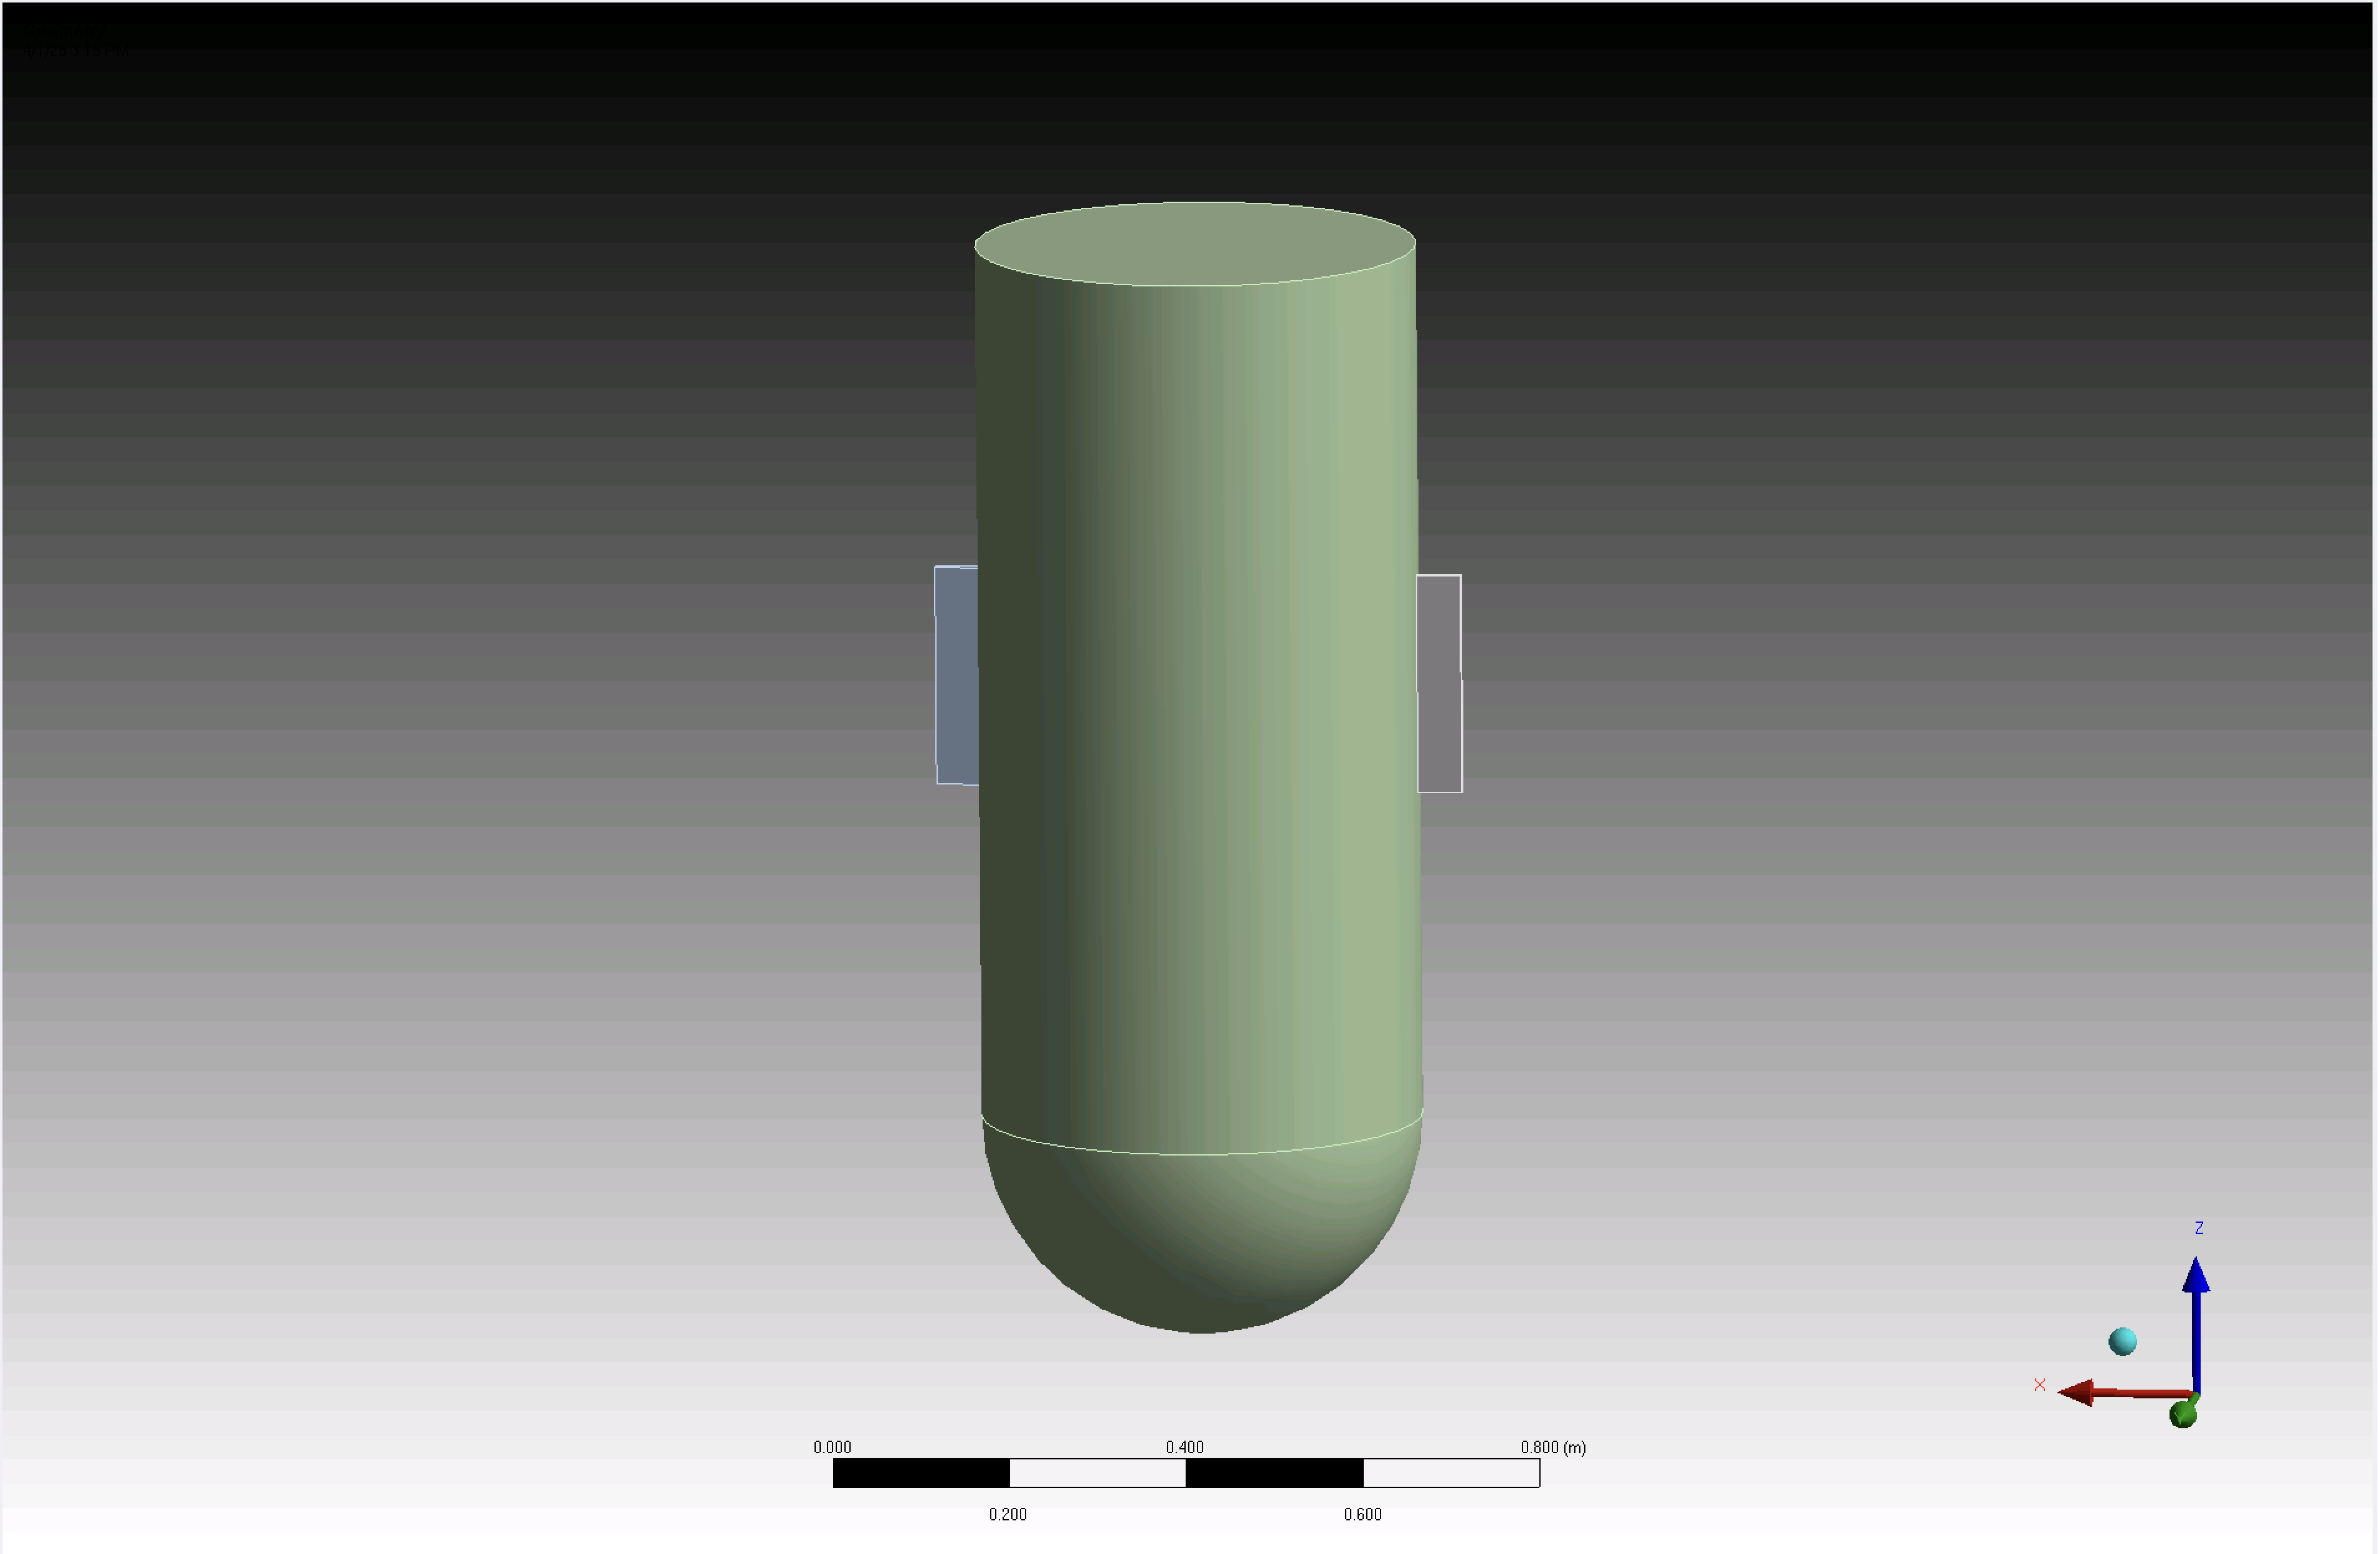
\includegraphics[width=0.65\textwidth]{img/geometry}
  \caption{Геометрiя ємностi з опорами (3D-вигляд у ANSYS SpaceClaim)}
\end{figure}

На зображеннi видно цилiндричну ємнiсть зi сферичним днищем та плоскою верхньою кришкою. Двi прямокутнi опори розташованi на зовнiшнiй цилiндричнiй поверхнi на серединi висоти.

\subsection{Розрахункова сiтка (Mesh)}

\begin{figure}[H]
  \centering
  \includegraphics[width=0.75\textwidth]{img/mesh}
  \caption{Розрахункова сiтка (Mesh), розмiр елемента 10~мм}
\end{figure}

На зображеннi видно цилiндричну ємнiсть зi сферичним днищем та плоскою верхньою кришкою. Опори розташованi на зовнiшнiй цилiндричнiй поверхнi на серединi висоти.

Сiтка: 255048 вузлiв, 166461 елементiв (SOLID187 тетраедри + SOLID186 гексаедри для контактних зон). Загальна маса моделi: 36{,}93~кг. Солвер: PCG (Preconditioned Conjugate Gradient), 4 ядра, збiжнiсть за 1729 iтерацiй, час розв'язання --- 64~с.

% ===================================================================
\section{Результати розрахунку}
% ===================================================================

Зведена таблиця результатiв:

\begin{table}[H]
  \centering
  \caption{Зведенi результати розрахунку}
  \begin{tabularx}{0.95\textwidth}{Xrrr}
    \toprule
    \textbf{Параметр} & \textbf{Мiнiмум} & \textbf{Максимум} & \textbf{Середнє} \\
    \midrule
    Total Deformation, м        & 0       & 0{,}42511   & 1{,}164$\times 10^{-2}$ \\
    Equiv.\ Elastic Strain, м/м & 7{,}258$\times 10^{-5}$ & 5{,}468$\times 10^{-2}$ & 3{,}316$\times 10^{-3}$ \\
    Equiv.\ Stress (von~Mises), Па & 1{,}135$\times 10^{7}$ & 9{,}912$\times 10^{9}$ & 4{,}694$\times 10^{8}$ \\
    \bottomrule
  \end{tabularx}
\end{table}

\subsection{Total Deformation}

\begin{figure}[H]
  \centering
  \includegraphics[width=0.85\textwidth]{img/deformation}
  \caption{Епюра сумарних деформацiй (Total Deformation) з маркером Maximum}
\end{figure}

Максимальне значення Total Deformation становить \textbf{425{,}1~мм} (0{,}425~м), мiнiмальне~--- 0 (у зонi фiксованих опор), середнє~--- 11{,}6~мм. Максимум спостерiгається у центрi плоскої верхньої кришки, де вiдсутнiсть кривизни не забезпечує жорсткостi оболонки. Цилiндрична стiнка та сферичне днище деформуються значно менше завдяки мембранному характеру їх напруженого стану.

\subsection{Equivalent Stress}

\begin{figure}[H]
  \centering
  \includegraphics[width=0.85\textwidth]{img/stress}
  \caption{Епюра еквiвалентних напружень (Equivalent Stress, von~Mises) з маркером Maximum}
\end{figure}

Максимальне значення Equivalent Stress (von~Mises) становить \textbf{9912~МПа} (9{,}91~ГПа), мiнiмальне~--- 11{,}3~МПа, середнє~--- 469~МПа. Максимум локалiзований у зонi переходу мiж плоскою кришкою та цилiндричною стiнкою. Концентрацiя напружень обумовлена рiзкою змiною кривизни оболонки у цьому мiсцi. На цилiндричнiй стiнцi напруження розподiленi бiльш рiвномiрно.

\subsection{Equivalent Elastic Strain}

\begin{figure}[H]
  \centering
  \includegraphics[width=0.85\textwidth]{img/strain}
  \caption{Епюра еквiвалентної пружної деформацiї (Equivalent Elastic Strain) з маркером Maximum}
\end{figure}

Максимальне значення Equivalent Elastic Strain становить \textbf{5{,}47$\times 10^{-2}$~м/м}, мiнiмальне~--- $7{,}26\times 10^{-5}$~м/м, середнє~--- $3{,}32\times 10^{-3}$~м/м. Розподiл деформацiй корелює з розподiлом напружень: максимум у зонi переходу кришка--стiнка.

% ===================================================================
\section{Аналiз та висновок}
% ===================================================================

Для оцiнки мiцностi порiвнюємо максимальне еквiвалентне напруження з межею текучостi:
\[
  \sigma_{\mathrm{eq,max}} = 9912~\text{МПа}
  \quad\text{vs}\quad
  \sigma_{\mathrm{yield}} = 207~\text{МПа}.
\]

Запас мiцностi:
\[
  n = \frac{\sigma_{\mathrm{yield}}}{\sigma_{\mathrm{eq,max}}}
    = \frac{207}{9912}
    = 0{,}021.
\]

Оскiльки $n = 0{,}021 \ll 1$, конструкцiя \textbf{не витримує} заданi навантаження. Критичним елементом є плоска верхня кришка товщиною лише 2{,}1~мм при дiаметрi 500~мм --- вона працює на згин i не може забезпечити необхiдну жорсткiсть при тиску 1{,}1~МПа.

Для порiвняння: аналiтична оцiнка максимального напруження у затисненiй круглiй пластинi
\[
  \sigma_{\max} = \frac{3 P R^2}{4 t^2}
    = \frac{3 \cdot 1{,}1 \cdot 248^2}{4 \cdot 2{,}1^2}
    \approx 11{,}5~\text{ГПа},
\]
що узгоджується з результатами чисельного моделювання (9{,}9~ГПа).

\textbf{Рекомендацiї:}
\begin{itemize}
  \item Замiнити плоску верхню кришку на сферичну або елiптичну для переведення навантаження iз згину у мембранний стан.
  \item Або збiльшити товщину плоскої кришки до $t \geq \sqrt{3PR^2 / (4\sigma_{\mathrm{yield}})} \approx 37$~мм.
\end{itemize}

% ===================================================================
\appendix
\section{Скрипт генерацiї геометрiї}
% ===================================================================

\subsection{common.py --- спiльна геометрiя ємностi}

\begin{lstlisting}[style=python]
"""Shared vessel geometry for Labs 1, 3, 5 (Variant 13).

Vessel specs:
  - Cylindrical shell: OD = 500 mm, wall = 2.1 mm, height = 1000 mm
  - Top lid: flat plate, thickness = 2.1 mm
  - Bottom lid: spherical (hemisphere), thickness = 2.1 mm
"""

import cadquery as cq

OD = 500.0
WALL = 2.1
ID = OD - 2 * WALL
R_OUT = OD / 2
R_IN = ID / 2
SHELL_H = 1000.0


def make_vessel_shell() -> cq.Workplane:
    outer_cyl = cq.Workplane("XY").circle(R_OUT).extrude(SHELL_H)
    inner_cyl = cq.Workplane("XY").circle(R_IN).extrude(SHELL_H)
    shell = outer_cyl.cut(inner_cyl)

    top_lid = (
        cq.Workplane("XY")
        .workplane(offset=SHELL_H)
        .circle(R_OUT)
        .extrude(WALL)
    )

    outer_sphere = cq.Workplane("XY").sphere(R_OUT)
    inner_sphere = cq.Workplane("XY").sphere(R_IN)
    hemisphere_shell = outer_sphere.cut(inner_sphere)
    cut_box = (cq.Workplane("XY")
        .box(OD + 10, OD + 10, OD + 10, centered=True)
        .translate((0, 0, (OD + 10) / 2)))
    hemisphere_shell = hemisphere_shell.cut(cut_box)

    vessel = shell.union(top_lid).union(hemisphere_shell)
    return vessel


def make_support_pads(n_pads=4, pad_w=50.0,
                      pad_h=50.0, pad_t=10.0):
    import math
    mid_z = SHELL_H / 2
    result = None
    for i in range(n_pads):
        angle_deg = 360.0 * i / n_pads
        pad = (
            cq.Workplane("XY")
            .workplane(offset=mid_z - pad_h / 2)
            .center(R_OUT + pad_w / 2, 0)
            .rect(pad_w, pad_t)
            .extrude(pad_h)
        )
        if angle_deg != 0:
            pad = pad.rotate((0, 0, 0), (0, 0, 1), angle_deg)
        if result is None:
            result = pad
        else:
            result = result.union(pad)
    return result
\end{lstlisting}

\subsection{lab1.py --- збiрка ємностi з опорами}

\begin{lstlisting}[style=python]
"""Lab 1 -- Static Structural analysis geometry (Variant 13).

Single body: cylindrical vessel shell with flat top lid,
spherical bottom lid, and 2 support pads fused into
the vessel wall. Exports as STEP.
"""

from pathlib import Path
import cadquery as cq
from common import make_vessel_shell, make_support_pads

vessel = make_vessel_shell()
pads = make_support_pads(n_pads=2, pad_h=250.0)
body = vessel.union(pads)

step_dir = Path(__file__).parent / "step"
step_dir.mkdir(exist_ok=True)
step_path = step_dir / "lab1.step"
cq.exporters.export(body, str(step_path))
\end{lstlisting}

\end{document}
